% !TeX root = ../main_paper.tex
% Section: Experiments and Results (Agent 1)
% Every number traces to COC_REPORT/build/v2/05_progress.md via _recon_content.md.

\section{Experiments}

\begin{table*}[t]
\centering
\footnotesize
\begin{tabular}{llcc ccccccc}
\toprule
Task & Obs & $|\mathcal{D}_0|$ & Init SR & Safe & Dropout & Ensemble & Thrifty & Stagger & Diff-DAgger & DISEIL (ours) \\
\midrule
GridWorld & state & 20 & 48.9 & 85.3$\pm$0.9 & 84.9$\pm$0.8 & 86.2$\pm$0.7 & 86.8$\pm$0.7 & 85.7$\pm$0.5 & -- & \textbf{92.4$\pm$0.4} \\
GridWorld & image & 20 & 47.0 & 88.8$\pm$0.9 & 88.4$\pm$0.7 & 88.8$\pm$0.9 & 88.7$\pm$0.6 & 89.1$\pm$0.8 & -- & \textbf{91.3$\pm$0.6} \\
Push-T & state & 20 & 46.2 & 82.0$\pm$3.0 & 84.8$\pm$2.7 & 85.9$\pm$2.6 & 83.2$\pm$3.2 & -- & 94.1$\pm$2.0 & \textbf{96.1$\pm$1.6} \\
Push-T & image & 20 & 43.3 & 78.1$\pm$3.5 & 82.1$\pm$3.1 & 83.2$\pm$3.0 & 79.3$\pm$3.6 & -- & 89.0$\pm$2.1 & \textbf{92.6$\pm$2.2} \\
Lift & state & 8 & 67.2 & 99.2$\pm$0.7 & 99.2$\pm$0.4 & 99.2$\pm$0.4 & \textbf{100.0$\pm$0.0} & -- & 99.2$\pm$0.4 & \textbf{100.0$\pm$0.0} \\
Lift & image & 8 & 66.4 & 99.6$\pm$0.4 & 97.2$\pm$1.6 & 98.8$\pm$0.7 & 99.6$\pm$0.4 & -- & 99.6$\pm$0.4 & \textbf{100.0$\pm$0.0} \\
Wipe & state & 12 & 47.7 & 88.0$\pm$1.1 & 88.6$\pm$1.8 & 86.8$\pm$1.9 & 89.0$\pm$1.1 & -- & 90.4$\pm$2.7 & \textbf{93.1$\pm$1.3} \\
Wipe & image & 12 & 45.2 & 69.6$\pm$2.4 & 83.2$\pm$3.0 & 84.4$\pm$3.2 & 69.2$\pm$4.0 & -- & 88.6$\pm$1.4 & \textbf{92.3$\pm$1.4} \\
Door & state & 4 & 56.8 & 91.8$\pm$2.1 & 92.5$\pm$1.2 & 88.8$\pm$3.1 & 89.6$\pm$1.7 & -- & 93.2$\pm$1.9 & \textbf{96.6$\pm$1.9} \\
Door & image & 4 & 43.1 & 82.4$\pm$1.4 & 81.8$\pm$1.5 & 83.0$\pm$4.9 & 82.8$\pm$1.2 & -- & 84.2$\pm$1.6 & \textbf{88.6$\pm$1.5} \\
\bottomrule
\end{tabular}
\caption{Final success rate (per cent) on held-out test episodes, meaning start
states never trained on. Mean $\pm$ standard error over 5 seeds (robot tasks) and
9 seeds (GridWorld), at a budget of 20 expert
demonstrations. $|\mathcal{D}_0|$ is the number of initial demonstrations and Init
SR the round-0 success rate. The highest mean in each row is in bold, ties bolded
jointly. Stagger allocates each round at random; the five DAgger baselines decide
when to query the expert. A dash marks a method that does not apply: Diff-DAgger
on GridWorld, whose policy is not a diffusion policy, and Stagger where it was not
run. The Lift rows sit at the 100 per cent ceiling, so the tie they show is not a
tie in sample efficiency. DISEIL reaches 100 per cent after the ninth
demonstration on Lift (state) and the seventeenth on Lift (image). ThriftyDAgger
needs the seventeenth on Lift (state).}
\label{tab:main}
\end{table*}

\begin{table}[tb]
\centering
\begin{tabular}{llcc}
\toprule
Task & Obs & Diff-DAgger & DISEIL \\
\midrule
Push-T & state & 1.57$\pm$0.49 & \textbf{2.81$\pm$0.93} \\
Push-T & image & 1.80$\pm$0.49 & \textbf{2.82$\pm$0.77} \\
Lift & state & 1.61$\pm$0.50 & \textbf{2.64$\pm$0.74} \\
Lift & image & 1.36$\pm$0.38 & \textbf{2.93$\pm$0.75} \\
Wipe & state & 1.43$\pm$0.36 & \textbf{2.91$\pm$0.90} \\
Wipe & image & 1.95$\pm$0.52 & \textbf{3.62$\pm$0.98} \\
Door & state & 1.84$\pm$0.50 & \textbf{3.43$\pm$0.95} \\
Door & image & 1.58$\pm$0.41 & \textbf{3.00$\pm$0.89} \\
\bottomrule
\end{tabular}
\caption{Per-demonstration information gain, mean $\pm$ standard error over the
same seeds: the policy's per-step loss on each newly acquired demonstration,
measured before retraining on it, with the higher value in bold. Diff-DAgger is
the one baseline that queries the expert on the same per-step loss the metric is
computed from, and it is lower in all eight settings in which it runs. GridWorld
is omitted because Diff-DAgger does not run there.}
\label{tab:infogain}
\end{table}

\begin{figure*}[t]
\centering
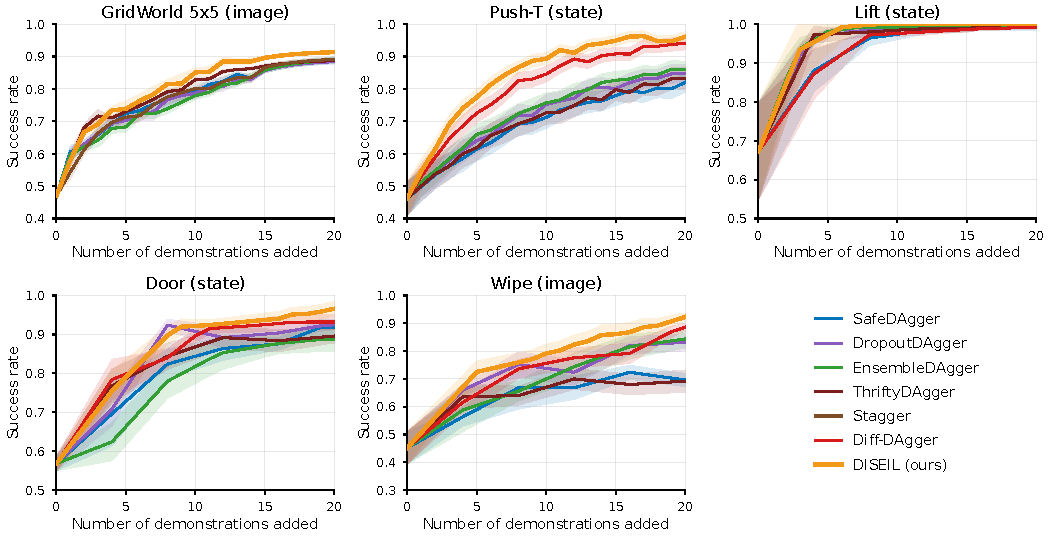
\includegraphics[width=\textwidth]{figures/learning_curves.pdf}
\caption{Held-out success rate against demonstrations acquired, mean $\pm$
standard error, on five settings spanning a discrete CNN policy and a continuous
diffusion policy.}
\label{fig:curves}
\end{figure*}

\subsection{Setup}

\noindent\textbf{Tasks and policies.}
We evaluate on five tasks. Each is run twice, with state observations and with
image observations, for ten settings in total. GridWorld is a $5 \times 5$
discrete grid with three obstacles. Push-T is the ManiSkill3 \texttt{PushT-v1}
environment \cite{tao2024maniskill3} of the task introduced by
\citet{florence2021implicitbc}; Lift, Wipe and Door are RoboSuite UR5/UR5e tasks
\cite{zhu2020robosuite}. Within a setting every method uses the same policy.
GridWorld (state) uses an MLP, GridWorld (image) a CNN. The four robot tasks use a
diffusion policy \cite{chi2023diffusionpolicy}, which takes images through an R3M
encoder \cite{nair2022r3m}. R3M supplies the policy's
features and never enters the partition, which is geometric in every run. The
expert is a human on GridWorld and a scripted or motion-planned oracle on Lift,
Door and Wipe. On Push-T the expert is a PPO policy \cite{schulman2017ppo} that
is competent in one rotational direction only. The task's constraint graph
excludes the configurations the expert cannot serve. No baseline can represent
that competence region, so part of DISEIL's Push-T margin may come from avoiding
expert failure rather than better allocation.

\noindent\textbf{Budget and measurement.}
Every method receives $B = 20$ expert demonstrations at $D = 1$ per round and
retrains on a shared cadence $m$, from scratch every round on GridWorld
($m = 1$) and on every fourth acquired demonstration on the robot tasks
($m = 4$). Three rounds in four therefore analyse a policy that has not been
refitted. Each still runs the policy on a fresh set of start states, so the
failure set and its partition are resampled rather than repeated. We report the
held-out success rate: the fraction of episodes solved on start states never
trained on. It is a mean $\pm$ standard error, $\mathrm{SE} =
\mathrm{std}/\sqrt{n}$, over $n = 9$ GridWorld seeds and $n = 5$ robot seeds. The
initial set
$|\mathcal{D}_0|$ is set per setting by a behaviour-cloning data-scaling sweep
targeting a round-zero success rate near 50 per cent, reported as Init SR in
Table~\ref{tab:main}. That band is where a fixed budget can be spent well or
badly: below it the failure set carries no structure, above it it is empty. The
ten settings are not ten independent experiments. A task's two settings share the
expert, the reward structure and the reset distribution, so the ten rows carry
less evidence than ten separate tasks would.

\noindent\textbf{Baselines.}
The comparison is against the query-efficient members of the DAgger family
\cite{ross2011dagger}: SafeDAgger \cite{zhang2017safedagger}, DropoutDAgger
\cite{menda2017dropoutdagger}, EnsembleDAgger \cite{menda2019ensembledagger},
ThriftyDAgger \cite{hoque2021thriftydagger} and Diff-DAgger
\cite{lee2025diffdagger}. All five decide only when to hand control to the expert,
each from a different score. None changes what the round's demonstration is spent
on. Diff-DAgger's score is the per-step denoising loss, the same signal DISEIL
uses to locate a failure; it runs on the robot tasks only. We add Stagger, a
control with no decision rule: it spends each round correcting one uniformly
chosen recorded failure. Running it on all eight robot settings was beyond the
compute available, so it exists on both GridWorld settings and, as ablation A2
below, on two robot settings. One asymmetry favours DISEIL. Its descriptor is read
from privileged simulator state, whereas the five baselines score the policy's own
output. The descriptor supplies only the partition, and no policy observes it.

\subsection{Main results}

\noindent\textbf{Highest mean in all ten settings.}
Table~\ref{tab:main} gives the final held-out success rate of every method. The
margin over the strongest baseline in each setting averages 2.80 percentage
points, with a standard deviation of 1.73 and a range from 0.0 to $+5.6$. The
strongest baseline
changes from row to row. It is Diff-DAgger on Push-T, Wipe and Door, under image
and state observations alike. On GridWorld it is ThriftyDAgger for state and
Stagger for image. On Lift (state) ThriftyDAgger ties DISEIL; on Lift (image)
three baselines are level at 99.6. The result rests on the margin recurring
across rows, not on its size in any one row. The standard errors across seeds
overlap in several rows, and no single row would support the claim on its own. On
GridWorld (image) the random control reaches 89.1 and the four
DAgger baselines 88.4 to 88.8. Deciding when to query the expert therefore buys
nothing there. DISEIL still gains 2.2 points, in line with the ablation below.

\noindent\textbf{Lift is at a ceiling, and the ceiling hides the result.}
DISEIL and ThriftyDAgger both reach 100.0$\pm$0.0 on Lift (state), so the row
reads as a tie. It is not one. DISEIL is at 100 per cent after the ninth
demonstration and ThriftyDAgger only after the seventeenth, so the same endpoint
costs eight fewer expert calls. On Lift (image) DISEIL reaches 100 per cent after
the seventeenth. A final number cannot express this once both methods have run
out of headroom. Lift also begins the budget furthest above the 50 per cent
target band, at 67.2 and 66.4. At a ceiling a null result cannot separate a
component that does nothing from one whose effect cannot be observed. The
ablation programme therefore runs only where headroom remains.

\noindent\textbf{Where the margin opens.}
Figure~\ref{fig:curves} tracks success rate against demonstrations acquired. On
Push-T the separation opens from about the fifth demonstration and holds, so
Table~\ref{tab:main} reports a gap present for three quarters of the run. On
GridWorld every method rises together and finishes bunched, so the $+2.2$ on
GridWorld (image) is among the smallest margins. Wipe (image) has not plateaued.
DISEIL and Diff-DAgger are still rising at the twentieth demonstration, so the
3.7-point gap rests on the final values, not on a demonstrated asymptote. A
longer budget could close it.

\subsection{Information gain}

Per-demonstration information gain is the policy's per-step loss on each newly
acquired demonstration, taken before the policy is retrained on it
(Table~\ref{tab:infogain}). Diff-DAgger is the reference here. It queries the
expert on the very loss the metric measures, so it is the one baseline that could
be expected to lead. It does not. DISEIL is higher in all eight settings in which
Diff-DAgger runs, higher than every other DAgger baseline in all ten, and higher
than Stagger in the four settings Stagger runs in (supplementary). DISEIL's own target
rule (Eq.~\ref{eq:target}) also selects on peak loss, so the metric is not neutral
to DISEIL either. The table establishes only that the acquired demonstrations are
not less informative. A high loss before retraining has two possible causes: the
demonstration is new to the policy, or it is incoherent. Incoherence is ruled out
by construction. An infeasible configuration never reaches the expert
(Eq.~\ref{eq:verify}), and the expert's own trajectories are the fitting target.
Two
readings survive that Table~\ref{tab:main} cannot separate: the demonstrations are
better, or the budget is better spread across the failures the policy is still
producing.
